% Template for Cogsci submission with R Markdown

% Stuff changed from original Markdown PLOS Template
\documentclass[10pt, letterpaper]{article}

\usepackage{cogsci}
\usepackage{pslatex}
\usepackage{float}
\usepackage{caption}

% amsmath package, useful for mathematical formulas
\usepackage{amsmath}

% amssymb package, useful for mathematical symbols
\usepackage{amssymb}

% hyperref package, useful for hyperlinks
\usepackage{hyperref}

% graphicx package, useful for including eps and pdf graphics
% include graphics with the command \includegraphics
\usepackage{graphicx}

% Sweave(-like)
\usepackage{fancyvrb}
\DefineVerbatimEnvironment{Sinput}{Verbatim}{fontshape=sl}
\DefineVerbatimEnvironment{Soutput}{Verbatim}{}
\DefineVerbatimEnvironment{Scode}{Verbatim}{fontshape=sl}
\newenvironment{Schunk}{}{}
\DefineVerbatimEnvironment{Code}{Verbatim}{}
\DefineVerbatimEnvironment{CodeInput}{Verbatim}{fontshape=sl}
\DefineVerbatimEnvironment{CodeOutput}{Verbatim}{}
\newenvironment{CodeChunk}{}{}

% cite package, to clean up citations in the main text. Do not remove.
\usepackage{apacite}

% KM added 1/4/18 to allow control of blind submission


\usepackage{color}

% Use doublespacing - comment out for single spacing
%\usepackage{setspace}
%\doublespacing


% % Text layout
% \topmargin 0.0cm
% \oddsidemargin 0.5cm
% \evensidemargin 0.5cm
% \textwidth 16cm
% \textheight 21cm

\title{Measuring Children's Early Vocabulary in Low-Resource Languages
Using a Swadesh-style Word List}


\author{{\large \bf George Kachergis* (kachergis@stanford.edu)}  \AND {\large \bf Alvin Wei Ming Tan* (tanawm@stanford.edu)} \AND {\large \bf Virginia A. Marchman (marchman@stanford.edu)}  \AND {\large \bf Michael C. Frank (mcfrank@stanford.edu)} \\ Department of Psychology, 450 Jane Stanford Way \\ Stanford, CA 94305 USA}

\newlength{\cslhangindent}
\setlength{\cslhangindent}{1.5em}

\begin{document}

\maketitle

\begin{abstract}
Early language skill is predictive of later life outcomes, and is thus
of great interest to developmental psychologists and clinicians. The
Communicative Development Inventories (CDIs), parent-reported inventories
of early-learned vocabulary items, have proven to be valid and reliable
instruments for measuring children's early language skill. CDIs have
been painstakingly adapted to dozens of languages, and cross-linguistic
comparisons thus far show both consistency and variability in language
acquisition trajectories. However, thousands of languages do not yet
have CDIs, posing a significant barrier to increasing the diversity of
languages that are studied. Here, we propose a method for selecting
candidate words to include on new CDIs, leveraging analysis of
psychometric properties of translation-equivalent concepts that are
frequently included on existing CDIs. Leveraging 26 datasets from
existing CDIs, we propose a list of 229 concepts that have low
variability in their cross-linguistic learning difficulty. This pool of
common concepts---analogous to the ``Swadesh'' lists used in
glottochronology---can be used as a starting point for future CDI
adaptations. We test how well the proposed list generalizes to data from
8 additional languages.

\textbf{Keywords:}
early language learning; CDI; psychometrics; cross-linguistic
comparison; Swadesh vocabulary
\end{abstract}

\hypertarget{introduction}{%
\section{Introduction}\label{introduction}}

Tools that enable valid assessments of children's early language
abilities are invaluable for researchers, clinicians and parents, as
early language skill is predictive of educational outcomes years later
(e.g., Bleses, Makransky, Dale, Højen, \& Ari, 2016). The
MacArthur-Bates Communicative Development Inventories (CDIs, Fenson et
al., 2007; Marchman, Dale, \& Fenson, 2023) are parent report
assessments that provide reliable and valid estimates of children's
early vocabulary size and other aspects of early communicative
development, such as use of gestures and of word combinations. Parent
report is a relatively quick and low-cost method to assess early
language skills as it takes advantage of the fact that parents are
``natural observers'' of their child's skills and does not depend on a
child engaging with an unfamiliar experimenter.

Over the years, the CDIs have been adapted to dozens of languages, with
forms now available in English, Spanish, French, Hebrew, and Mandarin,
to name just a few. Recently, data from more than 85,000 CDIs in 38
languages have been archived in a central repository (Wordbank, Frank,
Braginsky, Yurovsky, \& Marchman, 2017). These data have revealed both
cross-linguistic consistency and variability in early language skills,
with insights from these patterns informing theories of early language
learning (Frank, Braginsky, Yurovsky, \& Marchman, 2021). For example,
cross-linguistic analyses indicate that measures of vocabulary size are
tightly correlated with other aspects of early language skill, like
gesture and grammatical competence. Thus, over development, the language
system is ``tightly woven'' (Bates et al., 1994; Frank et al., 2021) and
early vocabulary size serves as a good proxy measure of children's
overall language skill.

On the CDIs, vocabulary size is assessed via a checklist format, which
enables caregivers to scan and recognize words their child produces or
understands, rather than relying on recall alone. For example, the
American English CDI Words \& Sentences (CDI:WS) form, targeting
children 16-30 months of age, is comprised of 680 words from 22 semantic
categories, including nouns (e.g., Body Parts, Toys, and Clothing),
action words, descriptive words, and closed-class words such as
pronouns. Items on this original CDI:WS were chosen to reflect a range
of difficulty levels (i.e., easy, moderate, and more difficult), as well
as capture the linguistic and societal contexts of (most) children
living in the US. Short versions of the CDI:WS forms are also available
(e.g., Fenson et al., 2000), consisting of a set of \(\sim100\) items
that generate scores that more strongly correlate with scores on the
long forms, while retaining representation across a broad set of
semantic categories.

Creating a new CDI requires a lot of effort and resources, presenting a
daunting barrier to increasing the diversity of languages studied.
Following the guidelines\footnote{\url{https://mb-cdi.stanford.edu/adaptations.htm}}
from the MacArthur-Bates CDI Advisory Board, the process of adapting a
CDI for a language other than American English goes well beyond simply
translating items on these forms to that new language. While the process
can begin with identifying translation equivalents (i.e., items that
capture the same general concept in both languages, e.g., ``dog'' in
English, and ``perro'' in Spanish), the final item set must then be
filtered so that all items appropriately reflect the linguistic and
sociocultural context of the children learning that language. This
process usually requires considerable time and effort by researchers who
are both native speakers of the language and who have experience with
children, to first select and identify translation equivalents and to
then iteratively add, refine, and pilot the new CDI in the target
language. Because the goal is to obtain the set of items that best
capture general trends and individual differences in that language, the
items across CDIs in different languages do not necessarily overlap to a
great extent. For example, the American English CDI:WS and Mexican
Spanish CDI:WS forms each have 680 words, but only have 463 overlapping
concepts (68\%).

It is well-established that, all over the world, early-learned words
reflect the people and things that children are likely to experience,
that is, words for family members, animals, and common household objects
(Frank et al., 2021; Tardif et al., 2008). Given this finding, it is
reasonable to ask: Is there a single set of translation equivalents that
would meet the criteria for inclusion on CDIs from multiple languages?

To facilitate this effort, it is useful to leverage Item-Response Theory
(IRT, Embretson \& Reise, 2013) models. IRT models infer both the
abilities of test takers and the difficulty of individual test items
(i.e., words), along standardized dimensions. Recent work using IRT
models has facilitated our understanding of the psychometric properties
of specific CDI instruments. As such, they offer the potential to not
only yield more accurate measures of children's language ability, but
also to enable the construction of language-specific Computerized
Adaptive Tests (CATs), which choose the next test item based on the
responses to the previous items, and thus quickly hone in on the test
taker's language ability. CAT-based CDIs presenting 50 or fewer items
have been found to strongly correlate with scores on the full CDI:WS
(Chai, Lo, \& Mayor, 2020; Makransky, Dale, Havmose, \& Bleses, 2016;
Mayor \& Mani, 2019). A general method for creating CDI CATs that work
well across a broader age range (12--36 months) has been proposed, and
tested for American English and Mexican Spanish (Kachergis, Marchman,
Dale, Mankewitz, \& Frank, 2022). However, the IRT model driving each
CAT needs to be trained on a large and normative dataset, which may not
be available in a given language. To date, the IRT models are fitted
separately for each language, and the fitted parameters (e.g., word
difficulty) are likely to vary across languages.

The goal of the current study is to use IRT modeling in conjunction with
data from Wordbank to examine whether there might be a core set of
concepts that are frequently included on CDIs,
and---importantly---whether enough of them are of roughly equal
difficulty across many languages to allow them to be used as candidate
items in new languages. This work takes its inspiration from the fields
of lexicostatistics and glottochronology, where researchers (notably,
Swadesh, 1971) have proposed lists of common concepts that exist in all
catalogued languages, in order to quantify the genealogical relatedness
and dates of divergence of languages. For example, the original Swadesh
list contains 100 words, comprised of categories including common
pronouns (\emph{I}, \emph{you}, \emph{we}), animals (\emph{man},
\emph{fish}, \emph{bird}, \emph{dog}), objects (\emph{tree},
\emph{leaf}, \emph{sun}, \emph{mountain}), and verbs (\emph{die},
\emph{see}, \emph{sleep}, \emph{kill}). Extending this work to the
development of a universal CDI, or ``Swadesh CDI,'' would include many
of the concepts that researchers have chosen to include on several
CDI:WS adaptations, and which have relatively similar difficulty across
many languages. If such a list were generalizable to other languages, it
could serve as a helpful starting point for the development of new CDI
adaptations, since the constituent words would already have good
cross-linguistic difficulty estimates.

In particular, our contributions are 1) to revise and extend a set of
translation-equivalent concepts in Wordbank, 2) to fit IRT models to 26
CDI:WS datasets, 3) to evaluate 25 candidate lists of Swadesh CDI items
from a cross-linguistic comparison of concept difficulty and inclusion,
4) to identify and characterize the most informative Swadesh CDI list of
229 concepts, and 5) to test its generalization to a set of eight
additional low-data languages. We then make a concrete proposal for how
this Swadesh CDI list could be used to create future CDI adaptations,
expanding the diversity of languages studied. We end by discussing the
strengths and weaknesses of our approach.

\hypertarget{methods}{%
\section{Methods}\label{methods}}

\hypertarget{item-response-theory}{%
\subsection{Item Response Theory}\label{item-response-theory}}

A variety of IRT models targeting different types of testing scenarios
have been proposed (see Baker, 2001 for an overview), but for the
dichotomous responses that parents make for each item (word) regarding
whether their child can produce a given word, we used the popular
2-parameter logistic (2PL) model that is best justified for CDI data out
of four standard models (see Kachergis et al., 2022).

The 2PL model jointly estimates for each child \(j\) a latent ability
\(\theta_j\) (here, language skill), and for each item \(i\) two
parameters: the item's difficulty \(b_i\) and discrimination \(a_i\),
described below. In the 2PL model, the probability of child \(j\)
producing a given item \(i\) is

\[P_{i}(x_i = 1 | b_{i},a_{i},\theta_j ) = \frac{1}{1 + e^{-D a_{i}(\theta_j - b_i )}}\]

where \(D\) is a scaling parameter (\(D=1.702\)) which makes the
logistic more closely match the ogive function used in a standard factor
analysis (Chalmers, 2012; Reckase, 2009). Children with high latent
ability (\(\theta\)) will be more likely to produce any given item than
children with lower latent ability, and more difficult items will be
produced by fewer children (at any given \(\theta\)) than easier items.
The discrimination (\(a_i\)) adjusts the slope of the logistic (in the
classic 1-parameter logistic ``1PL'' model, the slope is always 1).
Items with higher discrimination (i.e., slopes) better distinguish
children above vs.~below that item's difficulty level, and hence are
generally more useful. While other standard IRT models exist (e.g., the
3PL model adds a ``guessing'' parameter for each test item), a recent
study found the 2PL model most appropriate for multiple Wordbank
datasets (Kachergis et al., 2022).

\hypertarget{datasets}{%
\subsection{Datasets}\label{datasets}}

\begin{table}[H]
\centering
\begingroup\fontsize{9pt}{10pt}\selectfont
\begin{tabular}{lrr}
 {\textbf{Language}} & {\textbf{items}} & {\textbf{N}} \\ 
 Norwegian & 731 & 9304 \\ 
  English (American) & 680 & 8828 \\ 
  Danish & 725 & 3714 \\ 
  Portuguese (European) & 639 & 3012 \\ 
  Turkish & 711 & 2422 \\ 
  Spanish (Mexican) & 680 & 2025 \\ 
  Mandarin (Taiwanese) & 696 & 1897 \\ 
  English (Australian) & 558 & 1520 \\ 
  French (French) & 690 & 1410 \\ 
  Korean & 641 & 1376 \\ 
  Cantonese & 804 & 1295 \\ 
  German & 588 & 1181 \\ 
  Slovak & 609 & 1066 \\ 
  Mandarin (Beijing) & 799 & 1056 \\ 
  Russian & 728 & 1037 \\ 
  French (Quebecois) & 664 & 929 \\ 
  Swedish & 710 & 900 \\ 
  Spanish (Argentinian) & 699 & 784 \\ 
  Italian & 670 & 752 \\ 
  Spanish (European) & 588 & 593 \\ 
  Hebrew & 605 & 518 \\ 
  Latvian & 723 & 500 \\ 
  Czech & 553 & 493 \\ 
  Croatian & 717 & 377 \\ 
  Hungarian & 802 & 363 \\ 
  Dutch & 704 & 303 \\ 
   \hline
Greek (Cypriot) & 815 & 176 \\ 
  Spanish (Peruvian) & 600 & 105 \\ 
  Kigiriama & 696 & 100 \\ 
  English (Irish) & 660 & 99 \\ 
  Irish & 691 & 99 \\ 
  Kiswahili & 705 & 90 \\ 
  Finnish & 581 & 70 \\ 
  Persian & 558 & 50 \\ 
  \end{tabular}
\endgroup
\caption{CDI:WS items and subjects (N) per dataset. The final 8 datasets were used for a generalization test.} 
\end{table}

We report IRT analyses for twenty-six languages from Wordbank (Frank et
al., 2017), comprising production data from CDI:WS vocabulary checklists
that have at least 200 administrations.\footnote{\url{http://wordbank.stanford.edu/contributors}}
Data from the first twenty-six rows of Table 1 (Norwegian through Dutch)
were used to select a pool of words with approximately equal
cross-linguistic difficulty. CDI:WS production data from an additional
eight languages (bottom of Table 1: Greek through Persian) had too few
participants to be analyzed with IRT. Datasets for these languages were
used to test how well the selected pool can be expected to generalize to
new languages.

\hypertarget{uni-lemmas}{%
\subsubsection{Uni-lemmas}\label{uni-lemmas}}

Comparison across languages requires a method to map between words that
correspond to broadly similar concepts across languages. As such, each
item on the CDI:WS for each language was mapped onto a set of
``universal lemmas'' or ``uni-lemmas'', which are approximate
cross-linguistic conceptual mappings of words. For example, ``chat''
(French) and ``gato'' (Spanish) both correspond to the same uni-lemma,
\emph{cat}. These mappings were recently updated to improve their
quality and systematicity, and to increase coverage across items and
languages. This new set of uni-lemmas was constructed based on glosses
provided by the original contributors of the Wordbank datasets, which
were then verified by native or advanced proficient speakers of the
language, and cleaned to increase their consistency across languages.
All uni-lemmas are accessible from Wordbank; details about the recent
update can be found at
\url{https://github.com/langcog/update_unilemmas}.

\hypertarget{participants}{%
\subsubsection{Participants}\label{participants}}

The Wordbank datasets consisted of the CDI:WS production data for 48444
children aged 16--30 months on 23020 items across 34 forms. Note that
the distributions of demographic variables (age, sex, etc.) of these
datasets are not matched, so comparing overall language ability
estimates across languages would be ill-advised. (See Frank et al.
(2021) for a discussion of effects of demographic variables on
vocabulary development.) Thus, we focused only on the estimated item
parameters, and in particular the variability of item difficulty
(\(b_i\)).

\hypertarget{instruments}{%
\subsubsection{Instruments}\label{instruments}}

When a CDI:WS forms was administered, caregivers were asked to indicate
for each vocabulary item on the instrument whether or not their child
can recognizably produce (say) the given word in an appropriate context.

``Produces'' responses were coded as 1 and all other responses were
coded as 0. Our datasets consisted of a dichotomous-valued response
matrix for each language, of size \(N\) subjects \(\times\) \(W\) words.
All models, data, and code for reproducing this paper are available on
OSF\footnote{OSF repository:
  \href{https://osf.io/8swhb/?view_only=6f6ab9818f2a4bb288e05ca9e12f540c}{https://osf.io/8swhb/}.}.

\hypertarget{results}{%
\section{Results}\label{results}}

Across the 26 IRT models for different CDI:WS forms, difficulty and
discrimination parameters for a total of 23020 items were fitted. Of
those items, 95\% had uni-lemmas defined, with a median of 693 per
CDI:WS form (range: 553 in Czech to 804 in Cantonese). A total of 1839
uni-lemmas were defined across the 26 CDI:WS forms, but 528 of these
were singletons, appearing on only one of the 26
forms.\footnote{These singletons were significantly more difficult than the 1311 uni-lemmas appearing more than once ($M_1=$ 1.45; $M_{>1}=$ 0.85; $t(899)=7.66$, $p<.001$).}
There was a significant relation between how often a uni-lemma appears
and its difficulty: the more often a uni-lemma appears, the
\emph{easier} it tended to be (\(r=-0.37\), \(t(1837)=-17.15\),
\(p<.001\)). Moreover, there was a weak but significant relation between
the number of forms a uni-lemma appears on and its cross-linguistic
variability (\(r=0.17\), \(t(1309)=6.35\), \(p<.001\)). It is perhaps
intuitive that lower-variability items tend to be earlier-learned, and
are thus often selected to be on CDI forms, echoing prior work
characterizing the consistency of children's first words across several
languages (Tardif et al., 2008). However, these modest but significant
correlations were also important to keep in mind as we chose our Swadesh
CDI candidates, as selecting too many easy items could result in older
children being at ceiling.

\hypertarget{identifying-swadesh-cdi-candidates}{%
\subsection{Identifying Swadesh CDI
Candidates}\label{identifying-swadesh-cdi-candidates}}

The goal was to choose uni-lemmas with low variability in their
cross-linguistic difficulty---that is, uni-lemmas that are similarly
difficult to learn across languages. There were two thresholds that had
to be defined to select Swadesh CDI (S-CDI) candidates: 1) \(k\), the
number of current CDI:WS forms a uni-lemma must appear on, and 2)
\(v_{min}\), the threshold for variability in cross-linguistic
difficulty. For \(v_{min}\), we simply considered the uni-lemmas with a
variation in cross-linguistic difficulty that was half a standard
deviation less than average, among the set of uni-lemmas that were on at
least \(k\) forms. Assuming variability was normally-distributed, this
criterion preserved the least-variable 19\% of the uni-lemmas.

It was less clear how to choose \(k\), the minimum number of forms a
uni-lemma must appear on to be considered eligible. As reported above,
the more forms a uni-lemma appeared on, the easier that concept tended
to be, and the greater its cross-linguistic variability in difficulty
(\(SD(d)\)) tended to be. Thus, the higher the threshold \(k\), the more
bias there would be toward the Swadesh candidates being easier than
typical, as well as more variable in difficulty. Having a Swadesh CDI
list that was much easier than the CDI:WS is undesirable, as it may show
ceiling effects for older children, while selecting words that are more
variable in difficulty may result in a test that generalizes less well
to other languages. Of course, the higher \(k\), the fewer uni-lemmas
there were available to choose from: 1303 uni-lemmas appeared on 2 or
more CDIs, but only 30 appeared on all 26 CDIs.

Because choosing \(k\) is difficult \emph{a priori}, we opted to do a
grid search across all possible values. For each \(k\), we found the set
of \(N\) uni-lemmas appearing \(k\) times on each form, calculated the
mean and standard deviation of the difficulties of those items, and then
identified the subset of those \(N\) items with \(SD(d) < v_{min}\):
these comprised the \(k^{\textrm{th}}\) Swadesh list, as shown in Figure
1 (top). For each candidate Swadesh list, we evaluated the total test
information yielded by that Swadesh list for each of the 26 CDI:WS
forms. Total test information was calculated as the integral across a
range of test-taker abilities (here, \(\theta \in \{-4,4\}\)) of the
information yielded on a test, calculated using the IRT difficulty and
discrimination parameters for those test items. Finding the \(k\) that
yielded the highest total test information was the main objective (see
online Appendix for details).

As shown in Figure 1 (bottom), test information was maximized with
\(k=9\), and from these 1309 uni-lemmas appearing on at least 9 forms,
229 Swadesh-CDI items were selected for having cross-linguistic
variability below the threshold. The mean difficulty of the S-CDI items
was also quite close to the difficulty of the other uni-lemmas that
appeared on at least 9 forms (\(M(d_{Swad})=0.33\);
\(M(d_{other})=0.37\)), suggesting that the S-CDI items were fairly
representative.

\begin{CodeChunk}
\begin{figure}[tb]
\includegraphics{figs/grid-search-plots-1} \caption[Number of uni-lemmas appearing on at least $k$ lists (top)]{Number of uni-lemmas appearing on at least $k$ lists (top). Total test information for Swadesh lists, and random tests of the same length (bottom).}\label{fig:grid-search-plots}
\end{figure}
\end{CodeChunk}

\hypertarget{characterizing-the-swadesh-cdi}{%
\subsection{Characterizing the
Swadesh-CDI}\label{characterizing-the-swadesh-cdi}}

\begin{CodeChunk}
\begin{figure}[tb]

{\centering 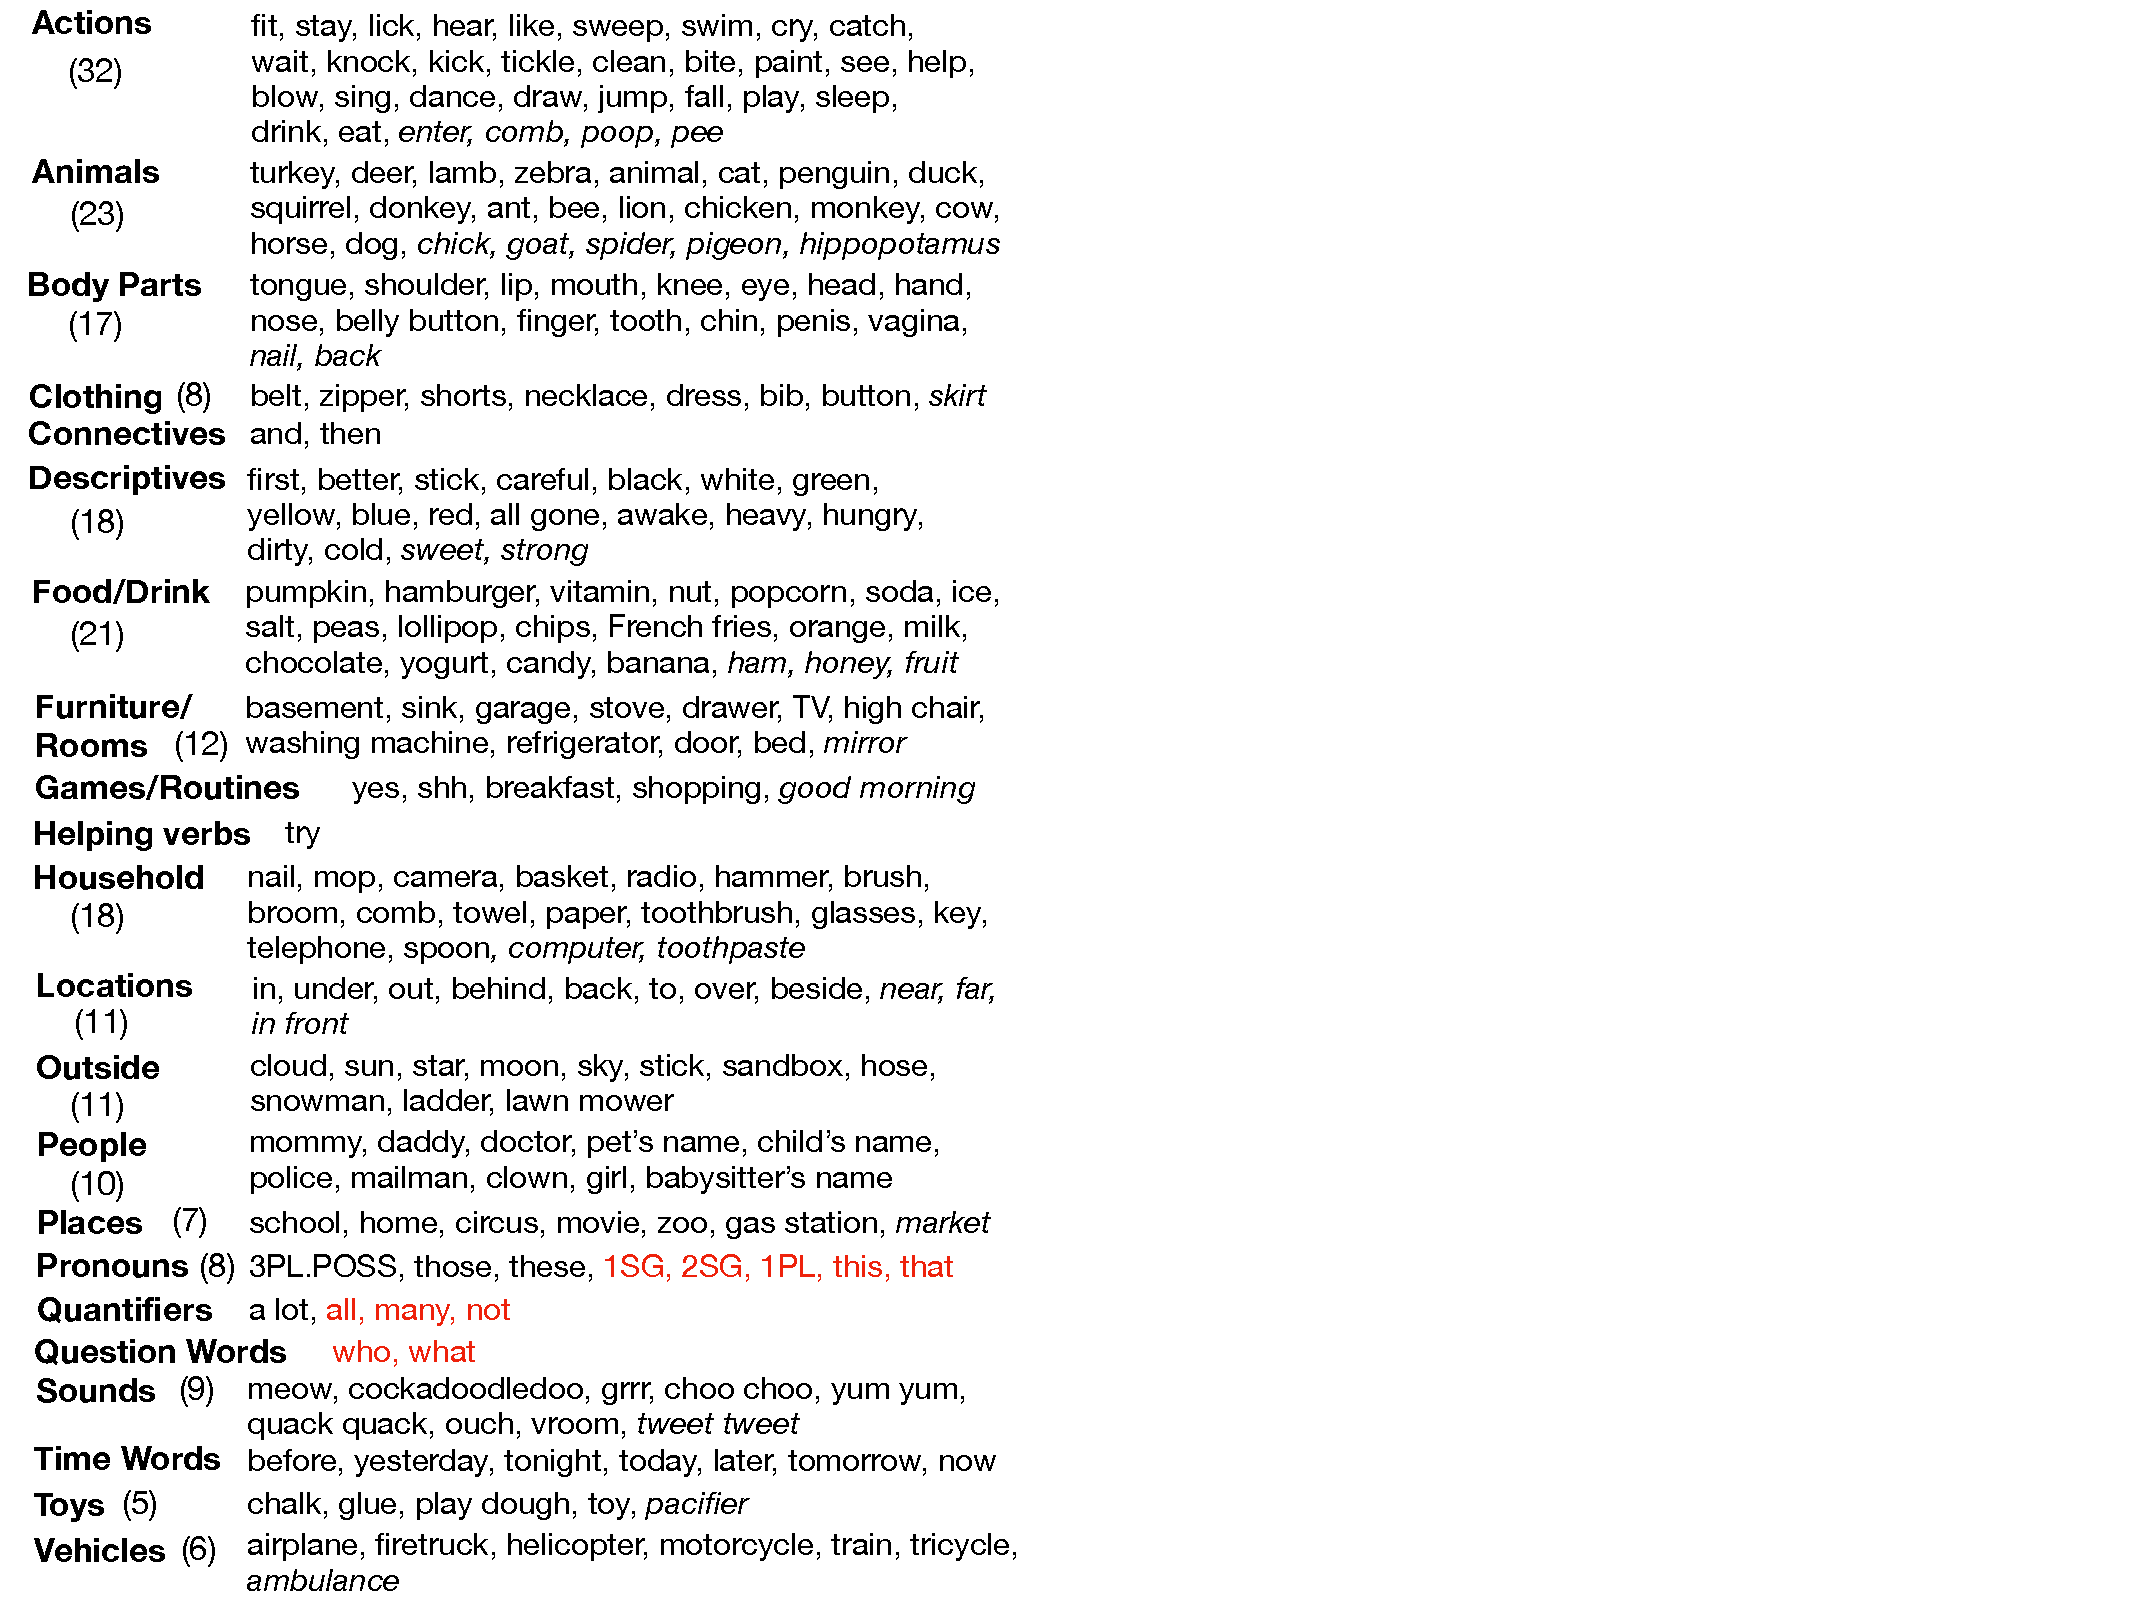
\includegraphics[width=\linewidth]{figs/SwadeshCDI_list} 

}

\caption[The 229 Swadesh CDI concepts by semantic category, and 10-item extension (in red)]{The 229 Swadesh CDI concepts by semantic category, and 10-item extension (in red). Italics denote the 28 items not included on the American English CDI:WS.}\label{fig:unnamed-chunk-5}
\end{figure}
\end{CodeChunk}

The 229 S-CDI items, shown in Fig. 3, represented 21 of the 22 semantic
categories present on the original American English CDI:WS form, with
concrete nouns, action words, and adjectives being most prevalent, and
connecting words, quantifiers, helping verbs, and articles being rare,
and question words being unrepresented (but see proposed extension
below). 54\% of the S-CDI concepts were nouns, 22\% were predicates
(verbs and adjectives), 17\% were function words, and 7\% belonged to
other lexical categories. This breakdown was comparable to the lexical
category percentages on the 680-item English CDI:WS (46\% nouns, 24\%
predicates, 15\% function words, and 5\% other), suggesting that the
S-CDI list did not show a particular lexical category bias. The S-CDI
items were also present on more forms than typical in the selection set:
on average, each item appeared on 19 forms, despite only being required
to appear on at least 9 forms. Finally, 28 S-CDI uni-lemmas were not
present on the American English CDI:WS (italicized in Fig. 3).

Figure 2 shows the average cross-linguistic difficulty of CDI items by
semantic category, for both Swadesh and non-Swadesh items. The
difficulty of Swadesh items generally tracked with that of non-Swadesh
items, although there were cases where one or the other was more or less
difficult.

\begin{CodeChunk}
\begin{figure}[h]

{\centering 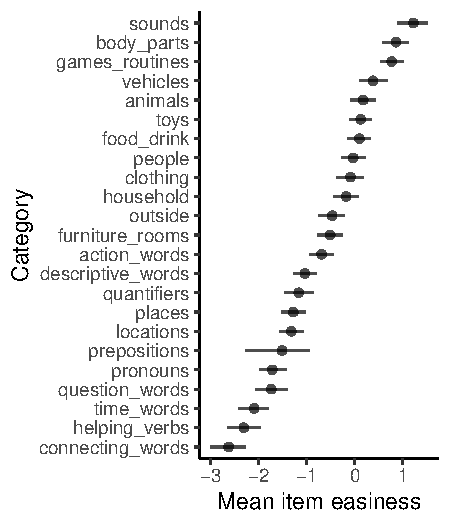
\includegraphics{figs/difficulty-by-category-1} 

}

\caption[Mean cross-linguistic difficulty of CDI words by semantic category, showing that selection of Swadesh concepts broadly maintained representative difficulty]{Mean cross-linguistic difficulty of CDI words by semantic category, showing that selection of Swadesh concepts broadly maintained representative difficulty. Bars represent bootstrapped 95\% confidence intervals.}\label{fig:difficulty-by-category}
\end{figure}
\end{CodeChunk}

Comparing the IRT parameters of the S-CDI uni-lemmas to the rest of the
items (across all CDI:WS forms) showed that the discrimination parameter
(i.e., slope) of the Swadesh items did not significantly differ from the
others, suggesting that the Swadesh items could measure ability as well
as non-Swadesh uni-lemmas. However, S-CDI items were significantly
easier than other uni-lemmas (mean S-CDI \(d=\) 0.11, others' mean
\(d=\) 0.53, \(t(8749)=-13.09\), \(p<.001\)).

To limit the likelihood of a ceiling effect, we proposed extending the
S-CDI with 10 additionanl uni-lemmas chosen from the original Swadesh
(1971) list, which were selected to fill gaps in the S-CDI, including
pronouns (\emph{I, you, we, this, that}), quantifiers (\emph{all, many,
not}), and question words (\emph{who, what}). These uni-lemmas are
included on a mean of 21 of the 26 forms, but are of greater difficulty
(mean \(d=0.84\)), and cross-linguistic variability (mean
\(sd(d)=1.36\)).

\hypertarget{validating-the-swadesh-cdi}{%
\subsection{Validating the Swadesh
CDI}\label{validating-the-swadesh-cdi}}

To validate the S-CDI, we first measured how well simulated raw scores
from the S-CDI items correlated with full CDI:WS scores. This metric
approximately reflects how reliable the S-CDI would be as a measure of a
child's vocabulary. On average, for the 26 large CDI:WS datasets, the
S-CDI's scores were strongly related to the full CDI:WS scores (mean
\(r=0.996\); \(min=0.989\), \(max=0.998\); full table on
\href{https://osf.io/8swhb/?view_only=6f6ab9818f2a4bb288e05ca9e12f540c}{OSF}).
We compared these correlations against a baseline that simulated an
upper bound for how well the Swadesh CDI could be expected to perform:
randomly sample \(N\) items from the actual CDI:WS of the target
language, where \(N\) is the number of Swadesh items that are present on
the form. On average, the 26 CDI:WS forms included \(N=176\) of the
Swadesh items.

Scores from a random subsample of CDI items tend to perform very well at
predicting the overall CDI score, as there are no sampling biases
related to item difficulty, or cross-linguistic variability in
difficulty or inclusion. However, note that this is \emph{not} a viable
method to create a new CDI, as in a true CDI construction scenario
rather than a simulation, the target CDI would not actually exist! Thus,
if the S-CDI comes close to performing as well as a random sample from
manually curated CDIs, we consider it a success. Indeed, the random
tests had a mean correlation with full CDI scores of \(r=0.997\), only
\(\epsilon=0.001\) higher than the S-CDI.

Next, we measured the total test information yielded by the two
baselines (recalling that total test information was one criterion for
the construction of the S-CDI). This metric reflects how well the S-CDI
would be able to differentiate the ability of children across different
ability levels. As reported above, the S-CDI yielded a mean total test
information of 66085, while the random uni-lemmas baseline yielded a
total test information of 66374. Although test information was slightly
lower for the S-CDI, the values were virtually indistinguishable.

\hypertarget{testing-generalization-of-the-swadesh-cdi}{%
\subsection{Testing Generalization of the Swadesh
CDI}\label{testing-generalization-of-the-swadesh-cdi}}

We then evaluated the S-CDI's performance in a test of generalization to
eight more CDI:WS datasets. For the eight low-data languages, a
comparison of simulated S-CDI scores to full CDI:WS revealed that the
S-CDI's raw scores were again strongly related (mean \(r=0.990\)), with
an average of \(N=153\) S-CDI items appearing per list. Table 2 shows
the results of this comparison, alongside the upper bound random
baseline. Once again, the S-CDI performed nearly as well as a random
sample of the actual CDI (random mean \(r=0.994\)). With the 10-item
extension, the S-CDI's correlation rose to mean \(r=0.993\),
demonstrating the value of including items from the more difficult (and
variable) categories that were underrepresented on the original list.

\begin{table}[H]
\centering
\begingroup\fontsize{9pt}{10pt}\selectfont
\begin{tabular}{lrrrr}
  \hline
language & N & Rand r & S-CDI r & S-CDI+10 r \\ 
  \hline
English (Irish) &  161 & 0.995 & 0.990 & 0.992 \\ 
  Finnish &  161 & 0.997 & 0.997 & 0.998 \\ 
  Greek (Cypriot) &  142 & 0.994 & 0.987 & 0.992 \\ 
  Irish &  160 & 0.995 & 0.988 & 0.994 \\ 
  Kigiriama &  179 & 0.996 & 0.996 & 0.997 \\ 
  Kiswahili &  179 & 0.996 & 0.992 & 0.992 \\ 
  Persian &  103 & 0.987 & 0.983 & 0.985 \\ 
  Spanish (Peruvian) &  141 & 0.996 & 0.991 & 0.993 \\ 
   \hline
\end{tabular}
\endgroup
\caption{Generalization test results for S-CDI vs. random baseline, and extended S-CDI (+10 items).} 
\end{table}

\hypertarget{discussion}{%
\section{Discussion}\label{discussion}}

This study compared psychometric models fitted to 26 CDI datasets in
order to find concepts that had low variability in their
cross-linguistic difficulty, and that were frequently included on CDI:WS
forms. We identified 229 concepts that appeared on at least 9 of the
CDIs, and which had more consistent cross-linguistic difficulty than
other concepts appearing on multiple CDIs. Using real-data simulations,
we showed that administering this set of Swadesh CDI items would
generate scores that were strongly related to full CDI:WS scores, both
for the original 26 datasets, and in a generalization test to eight
low-data languages. Moreover, the Swadesh CDI items resulted in
comparable total test information to tests of the same length composed
of randomly-selected uni-lemmas from the target test---a challenging
baseline to beat, and a construction method impossible to use when
creating a new CDI. The Swadesh CDI contains items with relatively
stable cross-linguistic difficulty estimates, and in the absence of
access to researchers who are familiar with relevant local cultures and
concepts, they may serve as a rapid, simple means of approximating
children's ability levels, even in the absence of a large norming
dataset.

However, the Swadesh CDI items were also significantly easier than other
items, meaning that older children may perform at ceiling if given only
the Swadesh CDI items. (This may be unsurprising from the perspective
that Swadesh words are meant to be universal, and are therefore more
frequent and basic---both within and across individual children's
experiences.) Thus, our suggested use case for the Swadesh CDI list is
as a starting point for researchers seeking to develop a CDI in a new
language, rather than as a complete short-form CDI based on existing
long-form CDI data. In particular, researchers should seek to add
relevant uni-lemmas from categories that were less well-represented on
the S-CDI, including question words, quantifiers, helping verbs, and
pronouns. These categories also tended to be more difficult, so adding
items from them is likely to increase the difficulty ceiling of the
form. Indeed, the inclusion of 10 such items drawn from the original
Swadesh (1971) list increased generalization performance.

Another potential limitation of this work is that most existing CDIs
(and most datsets available in Wordbank) target languages in the
Indo-European language family. It is not clear to what extent this bias
in the existing data might interfere with generalizing to
non-Indo-European languages. Nonetheless, our original 26 datasets
include 7 non-Indo-European languages (3 Sino-Tibetan, 1 Afro-Asiatic, 1
Uralic, 1 Koreanic, 1 Turkic), and the generalization datasets include 1
Uralic and 2 Niger-Congo languages (a language family not represented in
the original datasets); the broad consistency across language families
thus suggests that the effectiveness of the S-CDI may be sufficiently
robust.

Developing a list of appropriate vocabulary words is not the only
challenge researchers face when seeking to develop and use parent-report
measures in a new language and culture. The pragmatics of language
between children and adults can differ greatly across cultures, and has
been found to interfere with administration of parent-report measures of
early vocabulary, for example in Kiswahili (Alcock, 2017) and Wolof
(Weber, Marchman, Diop, \& Fernald, 2018). As such, local cultural
knowledge remains essential in appropriately developing and
administering novel CDI adaptations.

Despite the myriad challenges that remain in creating new measures of
early language development, we believe that the proposed Swadesh CDI
list will give researchers a solid foundation to start from, lowering
the barrier to the adaptation of CDI forms in new languages, since these
are often time-consuming and challenging to construct. Expanding the
number of languages with effective vocabulary measures would be a
critical step in addressing issues related to the under-representation
of lingustic diversity in language acquisition research (Kidd \& Garcia,
2022). Certainly, increasing the diversity of languages studied is a
critical step towards developing a truly general understanding of how
young children learn language.

\hypertarget{acknowledgements}{%
\section{Acknowledgements}\label{acknowledgements}}

Redacted for anonymous review.

\hypertarget{references}{%
\section{References}\label{references}}

\setlength{\parindent}{-0.1in} 
\setlength{\leftskip}{0.125in}

\noindent

\hypertarget{refs}{}
\leavevmode\vadjust pre{\hypertarget{ref-alcock2017production}{}}%
Alcock, K. J. (2017). Production is only half the story---first words in
two {East African} languages. \emph{Frontiers in Psychology}, \emph{8},
1898.

\leavevmode\vadjust pre{\hypertarget{ref-Baker2001}{}}%
Baker, F. B. (2001). \emph{The basics of item response theory}. ERIC.

\leavevmode\vadjust pre{\hypertarget{ref-bates1994}{}}%
Bates, E., Marchman, V., Thal, D., Fenson, L., Dale, P. S., Reznick, J.
S., \ldots{} Hartung, J. (1994). Developmental and stylistic variation
in the composition of early vocabulary. \emph{Journal of Child
Language}, \emph{21}(1), 85--123.

\leavevmode\vadjust pre{\hypertarget{ref-bleses2016}{}}%
Bleses, D., Makransky, G., Dale, P. S., Højen, A., \& Ari, B. A. (2016).
Early productive vocabulary predicts academic achievement 10 years
later. \emph{Applied Psycholinguistics}, \emph{37}(6), 1461--1476.

\leavevmode\vadjust pre{\hypertarget{ref-chai2020}{}}%
Chai, J. H., Lo, C. H., \& Mayor, J. (2020). A {B}ayesian-inspired item
response theory-based framework to produce very short versions of
{M}ac{A}rthur-{B}ates {C}ommunicative {D}evelopment {I}nventories.
\emph{Journal of Speech, Language, and Hearing Research}, \emph{63}(10),
3488--3500.

\leavevmode\vadjust pre{\hypertarget{ref-R-mirt}{}}%
Chalmers, R. P. (2012). {mirt}: A multidimensional item response theory
package for the {R} environment. \emph{Journal of Statistical Software},
\emph{48}(6), 1--29.
http://doi.org/\href{https://doi.org/10.18637/jss.v048.i06}{10.18637/jss.v048.i06}

\leavevmode\vadjust pre{\hypertarget{ref-embretson2013}{}}%
Embretson, S. E., \& Reise, S. P. (2013). \emph{Item response theory}.
Psychology Press.

\leavevmode\vadjust pre{\hypertarget{ref-Fenson2007}{}}%
Fenson, L., Marchman, V. A., Thal, D. J., Dale, P. S., Reznick, J. S.,
\& Bates, E. (2007). \emph{{M}ac{A}rthur-{B}ates {C}ommunicative
{D}evelopment {I}nventories: User's guide and technical manual (2nd
ed.)}. Baltimore, MD: Brookes.

\leavevmode\vadjust pre{\hypertarget{ref-Fenson2000}{}}%
Fenson, L., Pethick, S., Renda, C., Cox, J. L., Dale, P. S., \& Reznick,
J. S. (2000). Short-form versions of the {M}ac{A}rthur {C}ommunicative
{D}evelopment {I}nventories, \emph{21}, 95--116.

\leavevmode\vadjust pre{\hypertarget{ref-frank2017}{}}%
Frank, M. C., Braginsky, M., Yurovsky, D., \& Marchman, V. A. (2017).
Wordbank: An open repository for developmental vocabulary data.
\emph{Journal of Child Language}, \emph{44}(3), 677.

\leavevmode\vadjust pre{\hypertarget{ref-frank2021}{}}%
Frank, M. C., Braginsky, M., Yurovsky, D., \& Marchman, V. A. (2021).
\emph{Variability and consistency in early language learning: The
{Wordbank} project}. MIT Press.

\leavevmode\vadjust pre{\hypertarget{ref-Kachergis2022}{}}%
Kachergis, G., Marchman, V. A., Dale, P. S., Mankewitz, J., \& Frank, M.
C. (2022). Online computerized adaptive tests of children's vocabulary
development in {English} and {Mexican Spanish}. \emph{Journal of Speech,
Language, and Hearing Research}, \emph{65}(6), 2288--2308.

\leavevmode\vadjust pre{\hypertarget{ref-kidd2022}{}}%
Kidd, E., \& Garcia, R. (2022). How diverse is child language
acquisition research? \emph{First Language}, \emph{42}(6), 703--735.
http://doi.org/\href{https://doi.org/10.1177/01427237211066405}{10.1177/01427237211066405}

\leavevmode\vadjust pre{\hypertarget{ref-Makransky2016}{}}%
Makransky, G., Dale, P. S., Havmose, P., \& Bleses, D. (2016). An item
response theory-based, computerized adaptive testing version of the
{M}ac{A}rthur-{B}ates {C}ommunicative {D}evelopment {I}nventory: {W}ords
\& {S}entences ({CDI:WS}). \emph{Journal of Speech, Language, and
Hearing Research}, \emph{59}(2), 281--289.

\leavevmode\vadjust pre{\hypertarget{ref-marchman2023}{}}%
Marchman, V. A., Dale, P. S., \& Fenson, L. (2023).
\emph{MacArthur-bates communicative development inventories user's guide
and technical manual, 3rd edition}. Baltimore, MD: Brookes Publishing
Co.

\leavevmode\vadjust pre{\hypertarget{ref-mayor2019}{}}%
Mayor, J., \& Mani, N. (2019). A short version of the
{M}ac{A}rthur-{B}ates {C}ommunicative {D}evelopment {I}nventories with
high validity. \emph{Behavior Research Methods}, \emph{51}(5),
2248--2255.

\leavevmode\vadjust pre{\hypertarget{ref-reckase2009}{}}%
Reckase, M. D. (2009). Multidimensional item response theory models. In
\emph{Multidimensional item response theory} (pp. 79--112). Springer.

\leavevmode\vadjust pre{\hypertarget{ref-Swadesh1971}{}}%
Swadesh, M. (1971). \emph{The origin and diversification of language}.
(J. Sherzer, Ed.). Chicago, IL: Aldine.

\leavevmode\vadjust pre{\hypertarget{ref-tardif2008baby}{}}%
Tardif, T., Fletcher, P., Liang, W., Zhang, Z., Kaciroti, N., \&
Marchman, V. A. (2008). Baby's first 10 words. \emph{Developmental
Psychology}, \emph{44}(4), 929.

\leavevmode\vadjust pre{\hypertarget{ref-weber2018}{}}%
Weber, A. M., Marchman, V. A., Diop, Y., \& Fernald, A. (2018). Validity
of caregiver-report measures of language skill for {Wolof}-learning
infants and toddlers living in rural african villages. \emph{Journal of
Child Language}, \emph{45}(4), 939--958.
http://doi.org/\href{https://doi.org/10.1017/S0305000917000605}{10.1017/S0305000917000605}

\bibliographystyle{apacite}


\end{document}
